% ============================================================================
\section{From Separated Tracks to Conversation Understanding}
\label{sec:conversation}
% ============================================================================

A face-attributed, word-timed transcript is more than captions: it is the representation that ``who said what, when'' questions need, and the one that audio-only pipelines must first reconstruct by diarization. We built four uses on it---an interactive transcript, conversation insights, translated captions and grounded summaries---and measured each where a reference exists. All run on the same workstation at no recurring cost.

\subsection{Interactive transcript}
Every speaker's caption segments are merged into one conversation ordered by start time (Fig.~\ref{fig:conversation}a). Following playback, every line being spoken is highlighted, so during overlap two lines are active at once rather than one speaker being shown to hold the floor. Selecting a line switches the audio to that person's separated track and plays from the line's start: the transcript is a way to navigate the separation, not only to read it. Speakers can be renamed; names are stored with the project and applied to the manifest when it is served, so the player, transcript, exports and share pages read one source and the pipeline's output is never rewritten. The transcript can be searched (case- and accent-insensitive for Latin scripts; Indic scripts matched intact, since stripping combining marks changes words) and exported as SubRip, WebVTT with voice tags, plain text, or a Word document written in the browser.

\subsection{Conversation insights}
Speech is grouped into \emph{spurts}---a person's words joined across gaps of at most 0.5\,s. From spurts we report each person's talk time and share, turns, longest stretch and pace; \emph{overlap regions}, where two or more people speak for at least 250\,ms; and \emph{overlap onsets}, when B starts at least 200\,ms into A's spurt, classified following the distinction between cooperative and competitive overlap in meetings~\cite{shriberg2001overlap}: a \emph{backchannel} if B's spurt is shorter than 1\,s and ends inside A's, an \emph{interruption} if A stops within 2\,s and B outlasts A, and a \emph{talk-over} otherwise. The definitions are implemented twice---in Python for evaluation and in TypeScript in the browser---and both are pinned to one hand-computed fixture, so the numbers users see are the numbers measured here.

\textbf{Face-anchored diarization.} The captions' word timings answer \emph{who} well, because each track is bound to a face, but \emph{when} poorly: cross-track deduplication (Section~\ref{sec:amiav}) removes exactly the words spoken during overlap. An audio-only diarizer has the opposite profile---good boundaries, anonymous labels. We combine them. pyannote~3.1~\cite{bredin2020pyannote,plaquet2023powerset} segments the mixture into labelled turns; with $M_\ell$ the 10\,ms frames of label $\ell$ and $W_k$ those inside person $k$'s caption words, labels and people are paired one-to-one by
\begin{equation}
\pi^{*} = \arg\max_{\pi} \sum_{\ell} \lvert M_\ell \cap W_{\pi(\ell)} \rvert ,
\label{eq:anchor}
\end{equation}
solved with the Hungarian algorithm~\cite{kuhn1955hungarian}; a label left unpaired or paired with a person whose words it never overlaps is dropped rather than guessed. Every insight is then computed from the anchored turns, with word counts (for pace) from the captions.

\begin{table}[t]
\centering
\caption{Conversation insights on 30 AMI-AV meetings against the same insights from AMI's word alignments. MAE of talk share in percentage points (95\% bootstrap CI); F1 pooled over meetings. $^\ast$labels named by the reference, not achievable in a product.}
\label{tab:insights}
\footnotesize
\setlength{\tabcolsep}{3pt}
\begin{tabular}{@{}lccc@{}}
\toprule
& Talk share & Overlap & Interrupt. \\
System & MAE (pp) & F1 & F1 \\
\midrule
Caption words of the tracks & 13.1 {\scriptsize[10.2, 16.4]} & 0.38 & 0.07 \\
\textbf{Face-anchored diarization} & 12.9 {\scriptsize[9.0, 17.2]} & 0.77 & 0.21 \\
pyannote, oracle naming$^\ast$ & 6.4 {\scriptsize[4.6, 8.5]} & 0.77 & 0.33 \\
\bottomrule
\end{tabular}

\end{table}

Table~\ref{tab:insights} scores each design against the insights computed from AMI's hand-aligned words on all 30 meetings; an interruption counts as found if the same person interrupts the same person within $\pm$1\,s. Face anchoring doubles overlap F1 (0.38 to 0.77) and triples interruption F1 (0.07 to 0.21) at an unchanged talk-share error ($-0.2$ points, 95\% CI $[-2.7, +2.5]$). The pairing rule was chosen on the 20 fitting meetings only: one-to-one pairing beat giving each label to its best-overlapping person (talk-share MAE 11.3 against 15.4 points) and a Jaccard-normalised variant on every measure. On the ten held-out meetings the gains in overlap (0.80 against 0.42) and interruptions (0.11 against 0.08) held, but talk share was \emph{worse} than with caption words (16.1 against 13.1 points, $n{=}10$): when a label is paired with the wrong face, all of its talk time moves with it. The remaining gap to oracle naming ($+6.5$ points $[+3.2, +10.6]$) is that naming error, and it traces to visibility (Table~\ref{tab:amiav}): in TS3003a the most talkative participant's face is tracked for 11\% of the window, so their words---and the label they anchor---land on other faces. Overlap F1 is identical for the anchored and oracle systems because overlap regions do not depend on naming at all.

This complements, rather than contradicts, Section~\ref{sec:amiav}, where naming pyannote's clusters by face was worse for \emph{captions}. A caption must put each word under the right face, and a mislabelled cluster moves every word in it; deduplication decides word by word. Timing measures aggregate over frames and need boundaries the per-track words cannot give. Interruption detection remains weak for every system, oracle included (F1 0.33): AMI's interruptions are short and a 2\,s yield rule is coarse. The interface therefore presents interruptions and talk-overs as \emph{moments to review}, each playing the original mix from 1.5\,s before it (Fig.~\ref{fig:conversation}b).

\begin{figure*}[t]
\centering
\begin{minipage}[b]{0.235\textwidth}
\centering
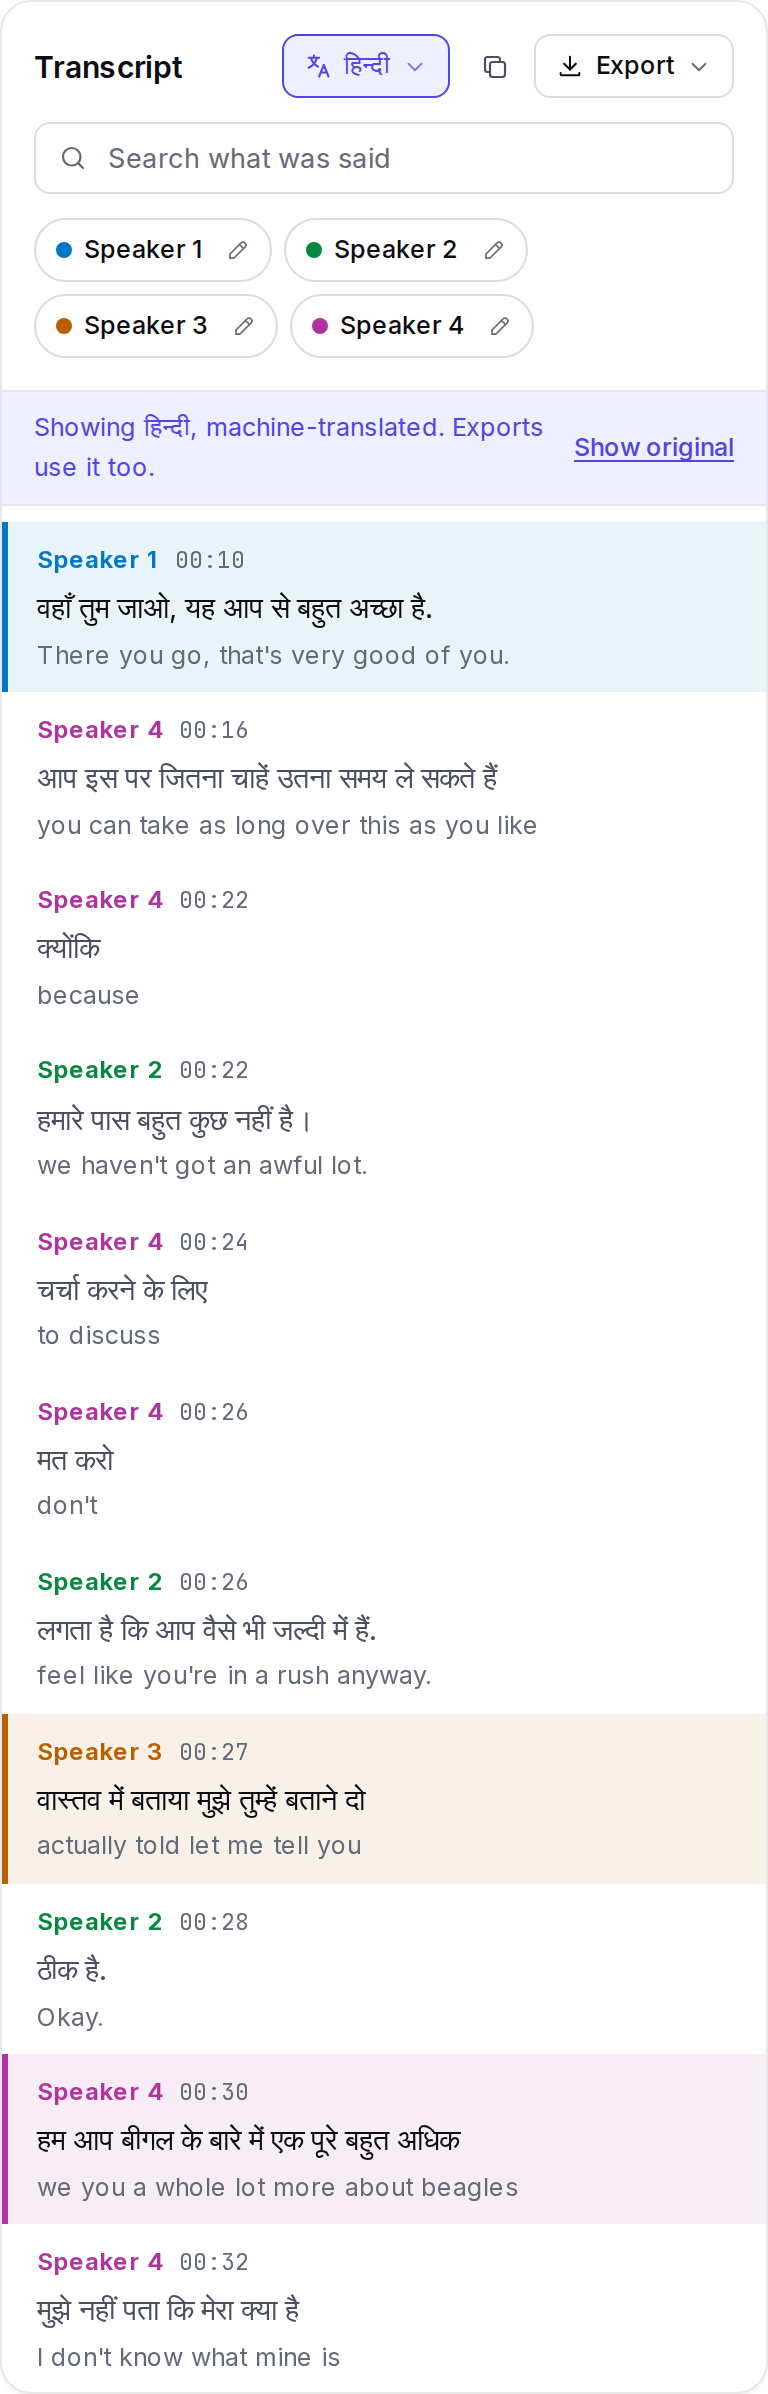
\includegraphics[width=\linewidth]{ui_transcript.png}\\[0.5mm]
\footnotesize (a) Transcript, read in Hindi
\end{minipage}\hfill
\begin{minipage}[b]{0.745\textwidth}
\centering
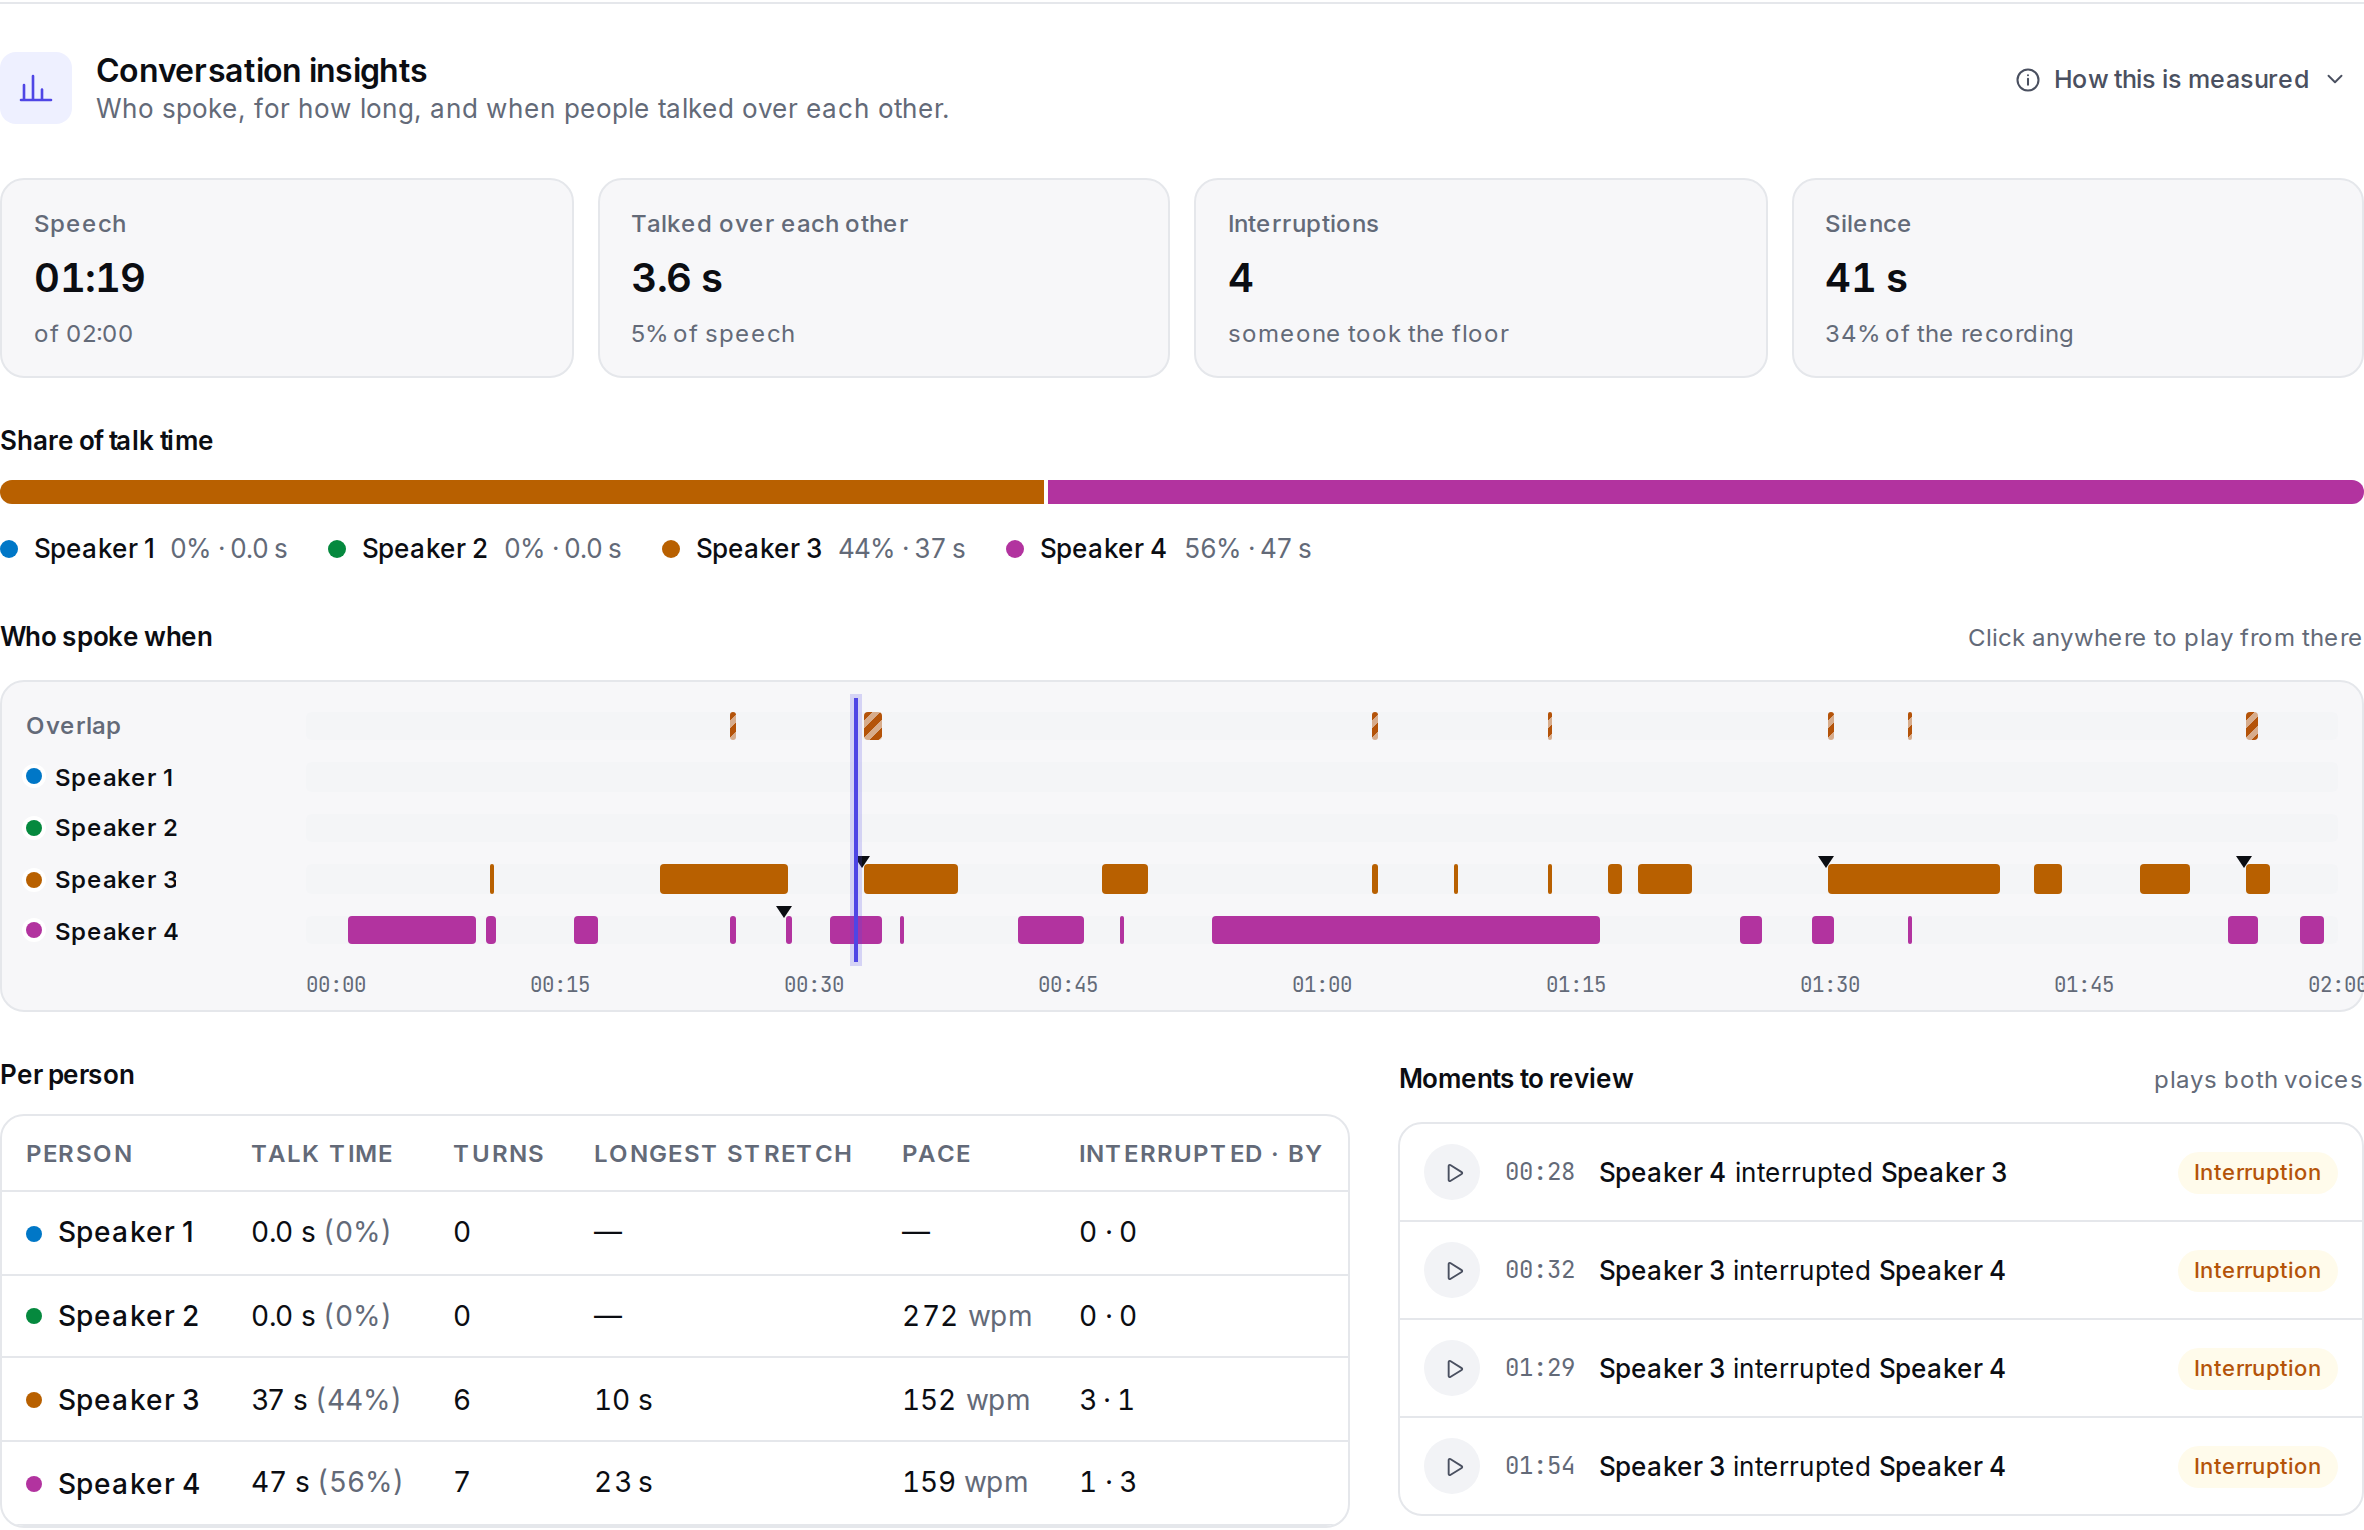
\includegraphics[width=\linewidth]{ui_insights.png}\\[0.5mm]
\footnotesize (b) Conversation insights
\end{minipage}
\caption{Conversation understanding in the production interface (live-site capture, AMI meeting ES2002a). (a) The merged transcript follows playback---during overlap both speakers' lines are highlighted---and is shown machine-translated into Hindi with the words as spoken beneath each line; selecting a line plays that person's separated voice. (b) Talk share, a who-spoke-when timeline with overlap regions, per-person statistics and moments to review, all from face-anchored diarization.}
\label{fig:conversation}
\end{figure*}

\subsection{Translated captions}
On request, every speaker's captions are translated by NLLB-200~\cite{nllb2024} (distilled 1.3B, pretrained, used as released under its non-commercial licence) through CTranslate2~\cite{ctranslate2} with 8-bit weights, the inference engine the recognizer already uses, so translation adds a model but no runtime dependency. Each caption segment is translated as one sentence and keeps its timing; word timings are dropped, since translation reorders words. The transcript, the player's caption and every export then read in the chosen language, with the original beneath each line (Fig.~\ref{fig:conversation}a). Forty target languages are offered, 18 of them scheduled languages of India, including four the recognizer cannot transcribe at all---Odia, Maithili, Kashmiri and Manipuri---so a meeting held in Kannada can be read in Odia. Every candidate target was screened by translating test sentences: Santali and Konkani produced SentencePiece unknown marks and untranslated English with the released model and are not offered, and the worker rejects any translation in which more than a fifth of the segments contain unknown marks. On the workstation, 100 caption segments translate in 0.7\,s once the model is loaded (4.7\,s, once per worker process). Translation quality is NLLB's own~\cite{nllb2024} and was not measured on this system.

\subsection{Summaries grounded in the transcript}
A summary---overview, key points, decisions and action items with owner and deadline---is written on request by Qwen2.5-7B-Instruct~\cite{qwen2025} (4-bit) served by Ollama~\cite{ollama} on the same GPU; nothing leaves the machine. Language models produce fluent text that is not always supported by their input; on the first trial, the model's overview said a speaker had lost weight, which nothing in the transcript states. We therefore require attribution in the spirit of citation-generation work~\cite{gao2023alce}: the prompt shows each line as \texttt{[L12 03:41 S2 Priya] text}, the answer is constrained to a JSON schema with bounded lists, and \emph{every} item, the overview included, must list the line ids it rests on. An item is kept only if at least one cited id is a real line, and an action item's owner must be one of the speakers or none. The page shows each item with play buttons for its cited lines, so the evidence is one click away. Long transcripts are summarised in parts of 220 lines; a part the model cannot answer within its token budget is halved, down to 30 lines.

\begin{table}[t]
\centering
\caption{Summaries of 30 AMI meetings from AMI's own speaker-attributed transcripts, against the action items and decisions AMI's annotators wrote. Lexical matching; a floor.}
\label{tab:summary}
\footnotesize
\setlength{\tabcolsep}{4pt}
\begin{tabular}{@{}lr@{}}
\toprule
Measure (30 meetings) & Value \\
\midrule
Meetings summarised / failed & 30 / 0 \\
Items citing no real line (dropped) & 0 of 314 \\
Action items P / R / F1 & 0.29 / 0.40 / 0.34 \\
\quad written / annotated / matched & 95 / 70 / 28 \\
Owner right (matched, role named) & 15 / 26 (58\%) \\
Decisions P / R / F1 & 0.00 / 0.00 / 0.00 \\
\quad written / annotated & 11 / 90 \\
Median time per meeting & 8.5\,s \\
\bottomrule
\end{tabular}

\end{table}

AMI's annotators recorded, for every scenario meeting, the actions agreed and the decisions taken, naming owners by role. We summarised each of the 30 meetings' \emph{whole} transcripts as AMI annotated them, with speakers named by role, and matched written items to annotated ones lexically (content words with role names removed, Dice overlap $\ge 0.35$, one-to-one), which undercounts paraphrases. This measures the summariser given a correctly attributed transcript; the separation's own errors are not compounded. Table~\ref{tab:summary} gives the result. Every meeting was summarised and no item had to be dropped for citing nothing real. Action items were found at a useful rate (recall 0.40, precision 0.29), and the owner was right for 15 of the 26 matched items that name a role (58\%; four roles, chance 25\%)---for example, the model's ``Review the user requirement specification'', owned by the Marketing Expert, against the annotators' ``The marketing expert will look at user requirement specifications'' (TS3005a). Many unmatched items are activities inside the meeting, such as AMI's warm-up exercise of drawing an animal, that annotators did not record as actions. Decisions were not found: the model wrote 11 against 90 annotated, and none matched. A median meeting took 8.5\,s.

\subsection{Shareable clips with burned-in captions}
People share moments, and video posted to feeds autoplays muted. An export can therefore be a clip---set by times, by the current playback position, or from transcript lines, where a second line stretches the clip---and can carry the captions in the picture, as spoken or in any translated language. Captions are written as ASS and drawn by ffmpeg's libass, which shapes Indic scripts with HarfBuzz; with several speakers each line leads with the name in that speaker's colour, and overlapping lines stack. A single-speaker export carries that speaker's captions only, matching its audio. Cutting or drawing requires re-encoding; the whole recording without captions is still a remux. In the end-to-end test, a 12\,s clip with Hindi captions was ready for download 4.3\,s after it was requested.
